\chapter{Orbital Perturbations}
\label{perturb}
\graphicspath{{chapter-3/Images/}}
%
% SRP - from "orbit mechanics about small asteroids"

% third body attraction - from wakker's astrodynamics notes page 540

% mass distribution effect from the asteroids itself (done through the harmonic expansion potential model) - so % this need not be covered again. but its important to identify the effect of asteroid's shape on the           % spacecraft's orbit. To consider the mass distribution effect we'll have to make use of the harmonics expansion % model for the potential.

% 'zonal maps' - topic of interest, read paper "orbital perturbation analysis near binary asteroid system" by   % chappaz and howell. Also third body disturbing function

% Lagrange planetary equations - one problem, the equation as defined in wakker's notes are for elliptical orbits, but what if the test particle in orbit is in an escape trajectory, then what happens? if the equations are not valid and suppose we have another set of equations for hyperbolic trajectory then how do we switch between the two? LPE is probably not the best thing to use as when dealing with multiple debris particles in orbit then all of them can have any type of orbit and if the type of orbit for each test debris will not be known previously, using LPEs might not be a nice idea then.

% Concept of averaging - needed for evaluating secular effect of perturbations, but is this relevant for the    % thesis or is it like overkill? - only do this when u do the thesis, not needed for literature survey

\section{Introduction}
Within the context of exploring the dynamic behavior of a particle near a pair of small irregular bodies, it is necessary to explore the effects of different perturbing forces, acting on the particle, on initial baseline orbits (orbits without perturbations). Perturbations hold significant importance especially when considering particle motion around small irregular bodies since the gravitational attraction of these bodies is weak relative to that of planets and thus even the smallest of the perturbing forces can result in drastic changes to baseline orbit designs. In this chapter we shall explore the perturbing forces of consequence in the context of a particle in motion around binary irregular asteroids.

\section{Solar Radiation Pressure}
\label{srp}
We begin with a simple model for the \gls{SRP} perturbation. The geometry involving the modeling of this perturbation is shown in \Cref{fig:srp}.

\begin{figure}[h]
\centering
\captionsetup{justification=centering}
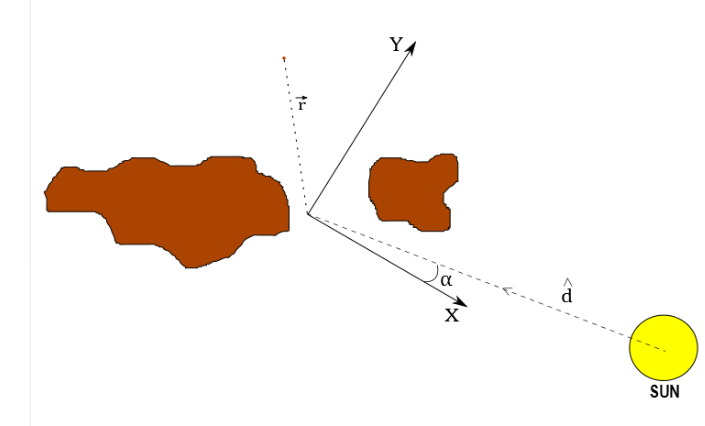
\includegraphics[scale=0.5]{srp2.png}
\caption{Geometry used in modeling \gls{SRP} perturbation. Diagram not to scale.}
\label{fig:srp}
\end{figure}
\FloatBarrier
%
The relative sizes and positions of the celestial bodies as depicted in \Cref{fig:srp} are not to scale and are shown therein for the purpose of representation only. The coordinate axis system as shown in the figure is an inertial frame with the origin attached to the barycentre of the binary asteroid system. The hidden axis, $Z$, completes the coordinate frame in the right hand sense and hence the axis is coming out of the plane of the figure. The unit vector, $\hat{d}$, points away from the sun and represents the inverse of the direction of the sun relative to the binary asteroid system. The angle $\alpha$ represents the longitude of the Sun with respect to the binary asteroid system. Note that the barycentre of the binary system is considered as the centre of the dynamical system shown in \Cref{fig:srp} and that the Sun is in a planar orbital motion around the centre. For simplicity, The motion of the Sun around the binary system is computed by solving the classical two-body point mass problem, the primary being the barycentre of the binary asteroid system and the secondary being the Sun. As we will see later, changing longitude of the Sun affects the direction in which the \gls{SRP} acceleration will be acting on a particle in orbit around the asteroids. Since only a planar system is considered here, the \gls{SRP} acceleration acting on an orbiting particle in the inertial $Z$ direction is null. The vector $\overrightarrow{r}$ depicts the inertial position of a particle in orbit around the asteroid system; note that this particle is in a proper three dimensional motion around the two asteroids. Another aspect to be noticed here is that the distance from the Sun to any particle in orbit around the binary asteroid system, is assumed to be the same as the distance between the Sun and the barycentre of the binary asteroids. This simplification was made because the distance to the Sun is extremely large compared to the distance between the orbiting particle and the barycentre and hence the position from the latter and the former to the Sun can be considered to be effectively equal.

The perturbing potential because of \gls{SRP} is given as \cite{dan_orb_mech}:
\begin{equation}
\label{srp_pot}
R_{SRP} = g_{SRP} \hat{d} \cdot \overrightarrow{r}
\end{equation}
%
where $g_{SRP}$ is the magnitude of the acceleration. Partial derivative of the perturbing potential $R_{SRP}$ with respect to the position vector $\overrightarrow{r}$ gives the perturbing acceleration vector as follows \cite{dan_orb_mech}:
\begin{equation}
\label{srp_acc}
\overrightarrow{g}_{SRP} = g_{SRP} \hat{d}
\end{equation}
%
where the magnitude of the acceleration is computed as follows \cite{dan_orb_mech}:
\begin{equation}
\label{srp_acc_mag}
g_{SRP} = \frac{\beta}{d^2}
\end{equation}
%
where $d$ is the magnitude of the distance between the centre of the Sun and the binary asteroid barycentre; the term $\beta$ is defined as follows \cite{dan_orb_mech}:
\begin{equation}
\beta = \frac{(1+\rho)G_1}{B}
\end{equation}
%
where B is the particle mass-to-area ratio in $\frac{kg}{m^2}$, $\rho$ is the reflectivity of the particle, and $G_1$ is the Solar constant and has a value of approximately $1\times10^8$ $\frac{kg\text{-}km^3}{s^2\text{-}m^2}$ \cite{dan_orb_mech}. The unit vector $\hat{d}$ is given as:
\begin{equation}
\label{d_unit}
\hat{d}
=
\begin{bmatrix}
-\cos(\alpha)\\
-\sin(\alpha)\\
0
\end{bmatrix}
\end{equation}
%
From \Cref{srp_acc} and \Cref{srp_acc_mag}, one can see that the magnitude of the perturbing acceleration depends on the distance to the Sun which varies all the time as the Sun traverses in an planar elliptic orbit around the binary asteroid system, and one can also infer that the direction of the perturbing acceleration changes with the longitude of the Sun with respect to the binary system. Note that the \gls{SRP} model presented here is very simple and is meant for discussions on bulk and qualitative effects of the perturbation. A detailed model will include the orientation of the asteroid's surface, it's temperature and a few other parameters \cite{scheeres_srp_regolith}.

For natural particles, such as the regolith on the surface of an asteroid, the reflectance $\rho$ of the particle is $<<1$ and hence, it can be assumed to be 0 \cite{scheeres_srp_regolith}. The particle is assumed to have a spherical shape with mass \textit{M} defined as $M = \frac{4 \pi \sigma r_0^3}{3}$ and total projected area $\pi r_0^2$, where $\sigma$ is the particle's density and $r_0$ is the particle radius \cite{scheeres_srp_regolith}. Thus for a spherical regolith particle the mass-to-area ratio $B$ is calculated as \cite{scheeres_srp_regolith}:
\begin{equation}
\label{regolith_B}
B = \frac{4 \sigma r_0}{3}
\end{equation}
%
As an example to understand the qualitative effect of \gls{SRP}, consider the regolith grain density of 2.5 $\frac{g}{cm^3}$ and particle grain radius of 0.2 micron for the asteroid Eros, which is at a distance of 1.13 AU \cite{scheeres_srp_regolith}. The magnitude of \gls{SRP} acceleration is then equal to $\mathbf{8.94 \times 10^{-3}}$ $m/s^2$. For Eros, with the gravitational parameter $\mu = 4.5 \times 10^{-4}$ $km^3/s^2$ and mean radius $R = 8.4$ km \cite{scheeres_srp_regolith}, the gravitational acceleration (assuming Eros to be a point-mass) is then equal to $\mathbf{6.38 \times 10^{-3}}$ $m/s^2$. It can be seen that for the given particle density and grain radius, the perturbing acceleration due to \gls{SRP} is of the same order of magnitude as the gravitational attraction of the asteroid, and hence \gls{SRP} can not be ignored whilst studying orbital motion of regolith around an asteroid.

\section{Third Body Perturbation}
\label{3bpert}
The presence of other celestial bodies, such as the Sun and Jupiter, will provide a perturbing force that will affect the motion of a particle in its orbit around the binary asteroid system. Let's denote the body or particle being perturbed with the index $i$, the perturbing bodies by index $j$, and the barycentre of the binary asteroid by the index $k$ which is also where the inertial reference frame is centered at. Then the perturbing potential as defined in this inertial reference frame is expressed by the following equation \cite{wakker}:
\begin{equation}
\label{3B_pert_pot}
R_{celt} = -G \sum_{j \neq i \text{,} k} m_j \left[ \frac{1}{r_{ij}} - \frac{\overrightarrow{r_i} \cdot \overrightarrow{r_j}}{r_j^3} \right]
\end{equation}
%
where $G$ is the universal gravitational constant; $m_j$ is the mass of the $j^{th}$ perturbing body; $r_{ij}$ is the distance between the bodies $i$ and $j$; $\overrightarrow{r_i}$ and $\overrightarrow{r_j}$ are the position vectors of the body $i$ and $j$ from the inertial reference frame as defined before; $r_j$ is the magnitude of the vector $\overrightarrow{r_j}$. A low-fidelity perturbing potential model will be considered, in the sense that the perturbing celestial bodies will be considered as point masses and that they are in planar elliptic motion around the binary asteroid system. The two celestial bodies which shall have considerable influence on the motion of a particle orbiting the asteroids, will be Jupiter and the Sun. The perturbing acceleration is defined as \cite{wakker}:
\begin{equation}
\label{3B_pert_acc}
g_{celt} = -\overrightarrow{\nabla} \left[ -Gm_j \left( \frac{1}{r_{ij}} - \frac{x_ix_j + y_iy_j}{r_j^3} \right) \right]
\end{equation}
%
The individual components of this perturbing acceleration, from \Cref{3B_pert_acc}, can be given as \cite{wakker}:
\begin{align}
\label{g_celt_x}
g_{celt\text{-}x} &= Gm_j \left( \frac{x_j - x_i}{r_{ij}^3} - \frac{x_j}{r_j^3} \right) \\
\label{g_celt_y}
g_{celt\text{-}y} &= Gm_j \left( \frac{y_j - y_i}{r_{ij}^3} - \frac{y_j}{r_j^3} \right) \\
\label{g_celt_z}
g_{celt\text{-}z} &= 0
\end{align}
%

To understand the qualitative effect of the gravitational attraction from a third body, we shall compute the gravitational acceleration from the Sun and Jupiter and compare it with the gravitational acceleration of the asteroid Eros. Since we want to look only at the qualitative effect, the distance between the perturbing third-bodies and the regolith particle will be assumed to be the same as the distance between the former and the asteroid Eros. This assumption is valid since the distance between an orbiting regolith particle and the asteroid will be relatively small compared to the distance between the perturbing third-bodies and the asteroid. The gravitational parameter of the sun is $1.327 \times 10^{20}$ $m/s^2$ \cite{mu_sun} and the distance to the asteroid from the sun is $1.13$ AU \cite{scheeres_srp_regolith} (Eros' perihelion distance \cite{eros_data}). Thus, the acceleration due to the Sun's gravitational pull (assuming point-mass attraction) is then equal to $\mathbf{4.64 \times 10^{-3}}$ $m/s^2$. The gravitational parameter for the Jupiter is $1.267 \times 10^{17}$ $m^3/s^2$ \cite{mu_jupiter}. Since we considered perihelion distance for Eros, we shall consider the perihelion distance for Jupiter (assuming a configuration where the Sun, Eros and Jupiter are in a straight line and in that order), which is $4.95$ AU \cite{mu_jupiter}. Then the distance between Eros and Jupiter is $3.82$ AU. Thus, the acceleration due to Jupiter's gravitational pull (assuming point-mass attraction) is then equal to $\mathbf{3.879 \times 10^{-7}}$ $m/s^2$. In \Cref{srp}, we calculated the gravitational attraction of Eros, which came out to be $\mathbf{6.38 \times 10^{-3}}$ $m/s^2$. Thus, the magnitude of perturbing acceleration from the Sun is of the same order of magnitude as the asteroid's gravitational acceleration. The magnitude of perturbing acceleration from the Jupiter, however, has an order four times less than the asteroid's gravitational acceleration and the Sun's perturbing acceleration.

\section{Lagrange Planetary Equations}
\label{sec:lpe}
When dealing with perturbed orbits, the classical orbital elements are no longer the constants of motion. In such a scenario, the orbital motion of a particle can be considered as a seamless transition from one set of orbital elements to another \cite{wakker}. For a given instant of time, if the corresponding Cartesian coordinates are converted to orbital elements, then for that instant of time, we speak of osculating elements \cite{wakker}. A set of first-order differential equations for the variation of the osculating elements with time, are termed as \gls{LPE} \cite{wakker}. For the motion of an orbiting particle, the effect of the perturbations is accounted for by entering them as a potential term, in addition to the gravitational potential, in the \gls{LPE}. By integrating the differential equations, the values for the osculating elements can be obtained for any instant of time \cite{wakker}. Thus, the variations in the osculating elements for a given integration time can provide valuable insight into how an orbit is being affected by the perturbing forces. The standard set of \gls{LPE} are given as follows \cite{scheeres2012orbit}:
\begin{align}
\frac{da}{dt} &= \frac{2}{na} \frac{\partial R}{\partial \chi} \\
\frac{de}{dt} &= \frac{1-e^2}{n a^2 e} \frac{\partial R}{\partial \chi} - \frac{\sqrt{1-e^2}}{na^2e} \frac{\partial R}{\partial \omega} \\
\frac{di}{dt} &= \frac{\cot{i}}{na^2\sqrt{1-e^2}}\frac{\partial R}{\partial \omega} - \frac{1}{na^2\sqrt{1-e^2}\sin{i}}\frac{\partial R}{\partial \Omega} \\
\frac{d\omega}{dt} &= \frac{\sqrt{1-e^2}}{na^2e}\frac{\partial R}{\partial e} - \frac{\cot{i}}{na^2\sqrt{1-e^2}} \frac{\partial R}{\partial i} \\
\frac{d\Omega}{dt} &= \frac{1}{na^2\sqrt{1-e^2}\sin{i}}\frac{\partial R}{\partial i} \\
\frac{d\chi}{dt} &= \frac{2}{na}\frac{\partial R}{\partial a} - \frac{1-e^2}{na^2e}\frac{\partial R}{\partial e}
\end{align}
where $a$ is the semi-major axis, $e$ is the eccentricity, $i$ is the inclination, $\omega$ is the argument of periapsis, $\Omega$ is the right ascension of the ascending node, $n$ is the mean motion and $\chi = -M_0$ where $M_0$ is the mean anomaly \cite{scheeres2012orbit}.

\section{Conclusion}
In this chapter, we covered the two most relevant sources of perturbation, i.e. \gls{SRP} and third-body gravitational attraction, that can effect the orbital motion of a particle around an asteroid. The perturbing effect of an asteroid's irregular shape will also be accounted for, since we will be using the polyhedron gravitational potential model (see \Cref{polyhedron}). For \gls{SRP}, we considered a low-fidelity perturbation model as a first step in analyzing its qualitative effect on baseline orbits of a particle.

We could have considered the method of \gls{LPE} in this literature study to better visualize the effects of perturbations on the orbital motion of the particle because the variation of Keplerian orbital elements is much more intuitive rather than the variation of Cartesian position and velocity components. Since we will be dealing with the orbital motion of regolith lofted from the surface of an asteroid, the analysis of which demands that we consider different initial conditions for the lofted particles which can lead to any type of orbit, then in this situation and under certain circumstances the \gls{LPE} method would lead to some singularities. For example, in case of orbits with very small inclination and/or eccentricity, the time derivatives of certain orbital elements would become infinitely large \cite{wakker}. Since we will be analyzing the orbits of multiple particles, some of which may have an escape trajectory, some may fall back to the asteroid's surface and some may remain in an orbit around the asteroid, the singularity problem may be encountered in case of the motion of one of those particles. This issue of singularity can be avoided by adopting a different set of orbital elements, however, even then we will have to consider certain special cases such as that of near-circular orbit or near-equatorial orbit and all of this will again not help in applying the \gls{LPE} method for a general analysis of particle orbital motion. Thus, for the aforementioned reasons, it was decided not to use \gls{LPE} for perturbation analysis.

Another method in which we can observe the variations in the classical orbital elements is by converting the Cartesian position and velocity vector for each epoch in the ephemeris of the particle's orbit around an asteroid to its equivalent orbital elements. The recorded values of the orbital elements for each epoch can then be plotted to observe their variation over a certain period of time.

One of the initial assumption made in this literature study is that some of the lofted regolith particles may escape from the gravitational attraction of the asteroid. These particles could first complete certain fixed number of orbits around the asteroid before escaping or they may escape without even completing a single orbit around the asteroid. Since there is a possibility that the lofted regolith may escape without completing even a single orbit, we can not use the averaging techniques to analyze the secular effects of orbit perturbations. This conclusion is a corollary from an earlier work in \cite{scheeres2012orbit} wherein averaging techniques were used to analyze the secular effects of perturbations for spacecraft orbits that complete a number of orbits around an asteroid and were assumed to not escape in general.

% The method of averaging has also not been considered here to analyze the secular effects of perturbations because, in this literature study, it is assumed that the regolith lofted from an asteroid's surface will be due to human space exploration activities and in this situation we are more concerned with the safety of the orbiting spacecraft which requires us to analyze the immediate short term effect of perturbations on particle orbital motion rather than long term secular variations.

% As a final point, we shall compare the (worst case) magnitude of the different perturbing forces that we have selected and infer on their relevance for future thesis work. Reference \cite{chappaz2015} provides coefficients that can be used to compare the relative strength of the standard perturbations out of which we'll compare the two which are relevant for our work namely the third body gravitational attraction from the sun and the solar radiation pressure. We have considered the asteroid Itokawa and a single debris of spherical shape with 1 cm radius. The coefficients are given as follows \cite{chappaz2015}:
% \begin{equation}
% \begin{aligned}
% C_t &= \frac{N^2}{n^2} \\
% C_g &= \frac{3gna^2}{2\mu}
% \end{aligned}
% \end{equation}
% %
% Where, $C_t$ is the coefficient for solar attraction perturbation and $C_g$ is the coefficient for the solar radiation pressure perturbation. Note that these coefficients do not give the magnitude of perturbation but the values obtained can be used to compare the strength of a perturbation relative to the other. The term $N$ denotes the mean motion of the asteroid around the sun; $n$ denotes the mean motion of the particle around the asteroid; $g$ denotes the solar radiation pressure force and is computed as $g = G_1B/R^2$ where $G_1 = 1\times 10^{14}$ $kgkm/s^2$, $B$ is the area-to-mass ratio, $R$ is the heliocentric distance of the asteroid; $a$ is the semi-major axis of the particle's orbit around the asteroid and $\mu$ is the gravitational parameter of the asteroid. Thus after inputting all the required values, we get the following two values for the coefficients as follows:
% \begin{equation}
% \begin{aligned}
% C_t &= 3.44 \times 10^{16} \\
% C_{g_p} &= 1.1169 \times 10^{-8} \\
% C_{g_a} &= 3.5309 \times 10^{-9}
% \end{aligned}
% \end{equation}
% %
% $C_{g_p}$ refers to the case when the asteroid is at the perhelion and similarly $C_{g_a}$ refers to the case where the asteroid is at aphelion. From the above strength coefficients, we can say that third body attraction from sun as a perturbing force is more significant than the solar radiation pressure acting on a small piece of dust.

Finally, we shall now bring together the results from the qualitative analysis of the different perturbing accelerations and compare them. The perturbing accelerations of \gls{SRP} and third-body gravitational attraction, along with the gravitational acceleration at the surface of an asteroid (assuming the asteroid is a point-mass), are given in \Cref{tab:perturbing_accelerations}.
%
\begin{table}[htb]
\centering
\caption{Comparison of the magnitudes of perturbing acceleration due to \gls{SRP} and third-body effect of the Sun and Jupiter with the magnitude of the acceleration due to gravity at the surface of asteroid Eros.}
    \begin{tabular}{ll}
    \hline
    Source                                  & Magnitude of acceleration [$m/s^2$]       \\
    \hline
    Solar Radiation Pressure                & $8.94 \times 10^{-3}$                     \\
    Third-body effect of the Sun            & $4.64 \times 10^{-3}$                     \\
    Third-body effect of the Jupiter        & $3.88 \times 10^{-7}$                     \\
    Acceleration due to gravity of Eros     & $6.38 \times 10^{-3}$                     \\
    \hline
    \end{tabular}
\label{tab:perturbing_accelerations}
\end{table}
%
We can observe that the magnitudes of the perturbing accelerations due to \gls{SRP} and the third-body effect of the Sun have the same order of magnitude as the acceleration due to gravity of Eros. Based on this qualitative analysis we should, in general, not ignore these two perturbing effects while analyzing the orbital motion of lofted regolith around an asteroid. The magnitude of perturbing acceleration due to the third-body effect of Jupiter has an order of magnitude which is 4 times smaller than the rest in \Cref{tab:perturbing_accelerations}, and as such can be ignored. Thus, the \gls{SRP} and the third-body effect of the Sun will be included as perturbing sources in the analysis of the orbital motion of lofted regolith around an asteroid.
